\subsection{Wireless Communication Channels}

Wireless communication channels provide the medium through which information is transmitted between communicating devices. Due to the random nature of the propagation environment, wireless signals are affected by various phenomena that influence transmission quality and system performance. Therefore, understanding the characteristics, impairments, and classification of wireless channels is essential for the design and analysis of modern communication systems.

\subsubsection{Wireless Channel Characteristics}

A wireless communication channel represents the physical medium through which electromagnetic waves propagate from a transmitter to a receiver. Unlike wired channels, where the transmission medium is fixed and relatively predictable, wireless channels are inherently dynamic and strongly influenced by the surrounding environment. Buildings, vehicles, terrain, and moving objects may alter the propagation path of transmitted signals, resulting in significant variations in the received waveform.

In communication theory, a wireless channel is commonly modeled as a linear system that modifies the transmitted signal during propagation. The received signal can generally be expressed as

\begin{equation}
y(t)=h(t)\ast x(t)+n(t)
\end{equation}

where $x(t)$ is the transmitted signal, $y(t)$ is the received signal, $h(t)$ denotes the channel impulse response, $\ast$ represents the convolution operation, and $n(t)$ denotes additive noise.

The channel impulse response contains information regarding the propagation environment and determines how the transmitted signal is transformed before reaching the receiver. Variations in the channel response arise from factors such as propagation distance, obstacles, mobility, and environmental conditions.

\begin{figure}[H]
    \centering

    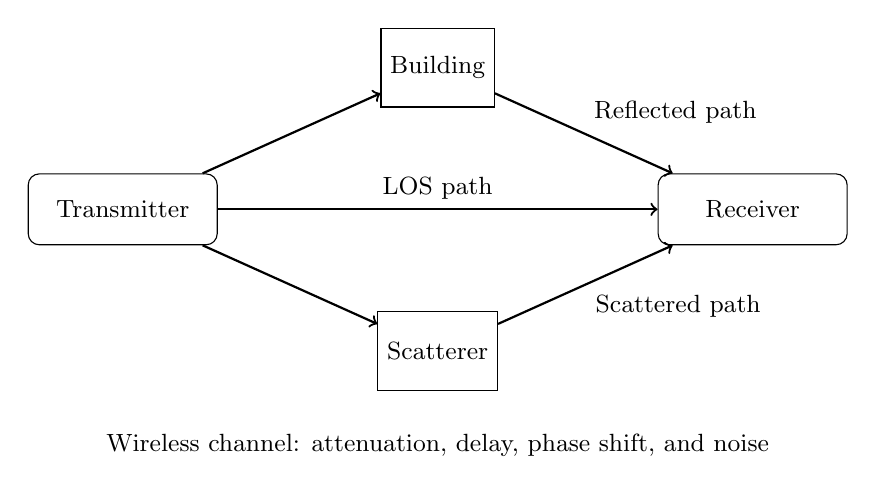
\begin{tikzpicture}[
        every node/.style={font=\small},
        block/.style={
            draw,
            rounded corners,
            minimum width=2.4cm,
            minimum height=0.9cm,
            align=center
        },
        obj/.style={
            draw,
            minimum width=1.2cm,
            minimum height=1.0cm,
            align=center
        },
        arrow/.style={->, thick}
    ]

    % Transmitter and receiver
    \node[block] (tx) at (0,0) {Transmitter};
    \node[block] (rx) at (8,0) {Receiver};

    % Objects
    \node[obj] (building) at (4,1.8) {Building};
    \node[obj] (scatterer) at (4,-1.8) {Scatterer};

    % Direct path
    \draw[arrow] (tx) -- node[above] {LOS path} (rx);

    % Reflected path
    \draw[arrow] (tx) -- (building);
    \draw[arrow] (building) -- node[above right] {Reflected path} (rx);

    % Scattered path
    \draw[arrow] (tx) -- (scatterer);
    \draw[arrow] (scatterer) -- node[below right] {Scattered path} (rx);

    % Channel label
    \node[align=center] at (4,-3.0)
    {Wireless channel: attenuation, delay, phase shift, and noise};

    \end{tikzpicture}

    \caption{General representation of a wireless communication channel.}
    \label{fig:wireless_channel_model}
\end{figure}

Figure~\ref{fig:wireless_channel_model} illustrates a typical wireless propagation scenario. Instead of following a single direct path, the transmitted signal may arrive at the receiver through multiple propagation paths generated by reflection, diffraction, and scattering mechanisms.

The unique characteristics of wireless channels distinguish them from wired transmission media. Signal attenuation increases with propagation distance, multiple signal replicas may be received due to multipath propagation, and mobility introduces time-varying channel behavior. These characteristics collectively create significant challenges for reliable wireless communication.

\subsubsection{Channel Impairments}

During propagation, wireless signals are subjected to various impairments that degrade transmission quality and limit communication performance. These impairments originate from the physical characteristics of the propagation environment as well as from practical limitations of communication hardware. Understanding their effects is essential for the design of reliable wireless transmission systems.

One of the most fundamental impairments is path loss, which refers to the gradual reduction in signal power as the propagation distance increases. In practical environments, obstacles such as buildings, vegetation, and terrain irregularities introduce additional attenuation, commonly known as shadowing. These effects reduce the received signal strength and may significantly limit communication coverage.

Another important impairment is multipath fading. Due to reflections, diffraction, and scattering, multiple copies of the transmitted signal arrive at the receiver through different propagation paths. Since these signal components experience different delays and phases, constructive and destructive interference may occur, leading to fluctuations in the received signal amplitude and phase.

Wireless communication systems are also affected by Doppler effects caused by relative motion between the transmitter, receiver, or surrounding scatterers. Doppler shifts introduce frequency offsets and time variations into the channel response, which become increasingly significant in high-mobility scenarios such as vehicular communications, high-speed railways, and unmanned aerial vehicle networks.

In addition, all practical receivers are affected by thermal noise generated by electronic components. This disturbance is commonly modeled as Additive White Gaussian Noise (AWGN) and represents a fundamental source of performance degradation in wireless communication systems.

\begin{figure}[H]
    \centering

    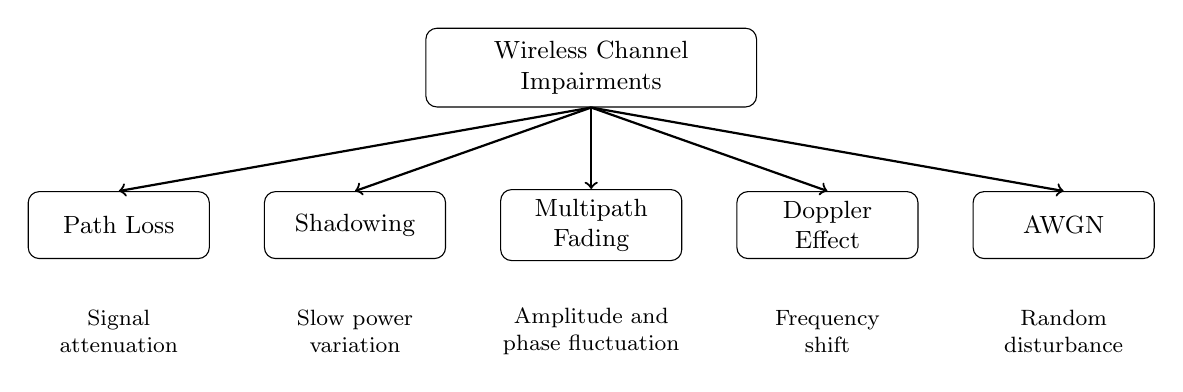
\begin{tikzpicture}[
        every node/.style={font=\small},
        main/.style={
            draw,
            rounded corners,
            minimum width=4.2cm,
            minimum height=1.0cm,
            align=center
        },
        item/.style={
            draw,
            rounded corners,
            minimum width=2.3cm,
            minimum height=0.85cm,
            align=center
        },
        desc/.style={
            align=center,
            font=\footnotesize
        },
        arrow/.style={->, thick}
    ]

    % Main node
    \node[main] (channel) at (0,0) {Wireless Channel\\Impairments};

    % Impairment nodes - increased spacing
    \node[item] (pathloss)  at (-6.0,-2.0) {Path Loss};
    \node[item] (shadowing) at (-3.0,-2.0) {Shadowing};
    \node[item] (multipath) at (0,-2.0) {Multipath\\Fading};
    \node[item] (doppler)   at (3.0,-2.0) {Doppler\\Effect};
    \node[item] (noise)     at (6.0,-2.0) {AWGN};

    % Arrows
    \draw[arrow] (channel.south) -- (pathloss.north);
    \draw[arrow] (channel.south) -- (shadowing.north);
    \draw[arrow] (channel.south) -- (multipath.north);
    \draw[arrow] (channel.south) -- (doppler.north);
    \draw[arrow] (channel.south) -- (noise.north);

    % Descriptions
    \node[desc] at (-6.0,-3.35) {Signal\\attenuation};
    \node[desc] at (-3.0,-3.35) {Slow power\\variation};
    \node[desc] at (0,-3.35) {Amplitude and\\phase fluctuation};
    \node[desc] at (3.0,-3.35) {Frequency\\shift};
    \node[desc] at (6.0,-3.35) {Random\\disturbance};

    \end{tikzpicture}

    \caption{Major impairments affecting wireless communication channels.}
    \label{fig:channel_impairments}
\end{figure}

The major impairments encountered in wireless communication channels and their corresponding effects are summarized in Table~\ref{tab:channel_impairments}.

\begin{table}[H]
\centering
\caption{Common wireless channel impairments and their effects.}
\label{tab:channel_impairments}

\begin{tabular}{|p{3cm}|p{4cm}|p{6cm}|}
\hline
\textbf{Impairment} &
\textbf{Primary Cause} &
\textbf{Effect on System Performance} \\
\hline

Path Loss &
Propagation distance &
Reduction of received signal power \\
\hline

Shadowing &
Obstacles and terrain &
Slow fluctuations in received signal strength \\
\hline

Multipath Fading &
Multiple propagation paths &
Amplitude and phase variations, signal distortion \\
\hline

Doppler Effect &
Relative motion &
Frequency shifts and channel time variations \\
\hline

AWGN &
Thermal noise &
Detection errors and performance degradation \\
\hline

\end{tabular}

\end{table}

The combined effects of path loss, fading, Doppler shifts, and noise represent the primary challenges faced by modern wireless communication systems. These impairments directly influence the design of modulation schemes, channel estimation algorithms, equalization techniques, and receiver architectures. Consequently, accurate channel modeling is a crucial step in the development and evaluation of advanced communication technologies.


\subsubsection{Channel Classification}

Wireless communication channels can be classified according to different characteristics of the propagation environment. Such classifications provide useful insight into channel behavior and help communication engineers select appropriate transmission and receiver techniques for specific operating conditions.

Based on frequency selectivity, wireless channels are generally categorized as flat-fading channels or frequency-selective channels. In a flat-fading channel, all frequency components of the transmitted signal experience approximately the same channel gain and phase shift. Conversely, a frequency-selective channel affects different frequency components differently, resulting in signal distortion and potential inter-symbol interference.

From a temporal perspective, channels may be classified as time-invariant or time-varying. A time-invariant channel remains relatively stable during the transmission interval, whereas a time-varying channel exhibits continuous fluctuations due to user mobility and changes in the propagation environment.

Wireless channels can also be categorized according to propagation conditions. Line-of-Sight (LOS) channels contain a direct propagation path between the transmitter and receiver, while Non-Line-of-Sight (NLOS) channels rely mainly on reflected, diffracted, and scattered signal components.

Table~\ref{tab:channel_classification} summarizes several common criteria used for wireless channel classification.

\begin{table}[H]
\centering
\caption{Classification of wireless communication channels.}
\label{tab:channel_classification}

\begin{tabular}{|p{4cm}|p{4cm}|p{4cm}|}
\hline
\textbf{Classification Criterion} &
\textbf{Category 1} &
\textbf{Category 2} \\
\hline

Frequency Selectivity &
Flat Fading &
Frequency Selective \\
\hline

Time Variation &
Time Invariant &
Time Varying \\
\hline

Propagation Condition &
LOS &
NLOS \\
\hline

Mobility Scenario &
Low Mobility &
High Mobility \\
\hline

\end{tabular}

\end{table}

\begin{figure}[H]
    \centering

    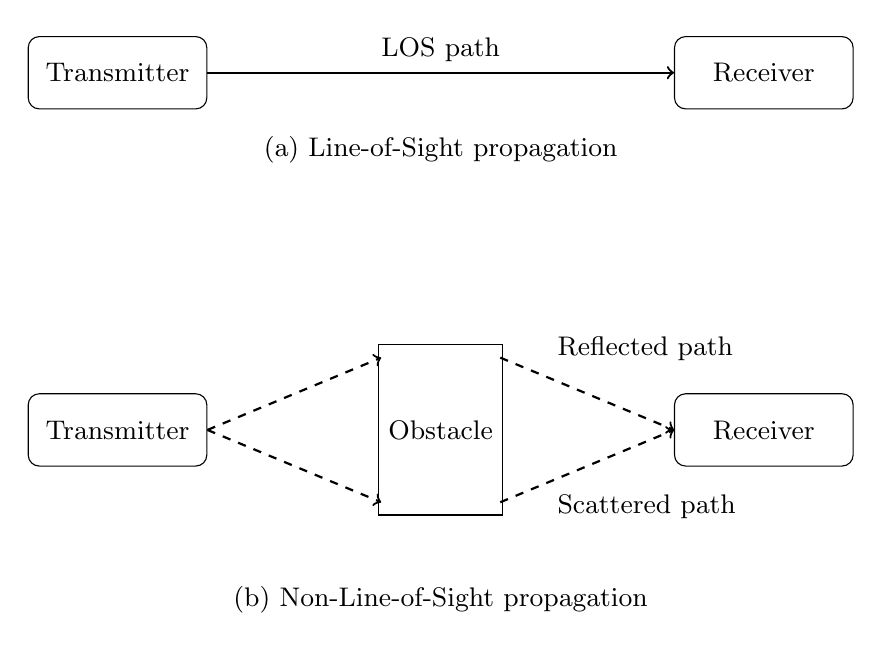
\begin{tikzpicture}[
        scale=1.08,
        transform shape,
        every node/.style={font=\small},
        device/.style={
            draw,
            rounded corners,
            minimum width=2.1cm,
            minimum height=0.85cm,
            align=center
        },
        obstacle/.style={
            draw,
            minimum width=1.45cm,
            minimum height=2.0cm,
            align=center
        },
        arrow/.style={->, thick},
        dashedarrow/.style={->, thick, dashed}
    ]

    % =========================
    % LOS scenario
    % =========================
    \node[device] (tx1) at (0,2.2) {Transmitter};
    \node[device] (rx1) at (7.6,2.2) {Receiver};

    \draw[arrow] (tx1.east) -- node[above] {LOS path} (rx1.west);

    \node[align=center] at (3.8,1.3) {(a) Line-of-Sight propagation};

    % =========================
    % NLOS scenario
    % =========================
    \node[device] (tx2) at (0,-2.0) {Transmitter};
    \node[obstacle] (obs) at (3.8,-2.0) {Obstacle};
    \node[device] (rx2) at (7.6,-2.0) {Receiver};

    % Points near obstacle edges (shorter dashed arrows)
    \coordinate (topL) at (3.1,-1.15);
    \coordinate (topR) at (4.5,-1.15);
    \coordinate (botL) at (3.1,-2.85);
    \coordinate (botR) at (4.5,-2.85);

    % Dashed paths
    \draw[dashedarrow] (tx2.east) -- (topL);
    \draw[dashedarrow] (topR) -- (rx2.west);

    \draw[dashedarrow] (tx2.east) -- (botL);
    \draw[dashedarrow] (botR) -- (rx2.west);

    % Labels moved away from paths
    \node[anchor=west] at (5.05,-1.05) {Reflected path};
    \node[anchor=west] at (5.05,-2.9) {Scattered path};

    \node[align=center] at (3.8,-4.0) {(b) Non-Line-of-Sight propagation};

    \end{tikzpicture}

    \caption{Illustration of LOS and NLOS propagation scenarios.}
    \label{fig:los_nlos}
\end{figure}

Among the various channel categories, high-mobility wireless channels represent one of the most challenging communication environments. In such scenarios, the channel often exhibits both frequency selectivity due to multipath propagation and time selectivity due to Doppler effects. These characteristics lead to the so-called doubly selective channel, which plays a central role in the development of advanced waveform technologies such as OTFS. The propagation mechanisms responsible for these effects are discussed in the following section.
